\documentclass{beamer}

\usefonttheme{professionalfonts} % using non standard fonts for beamer
\usefonttheme{serif} % default family is serif

%\usepackage{hyperref}

%\usepackage{minted}

\usepackage{animate}

\usepackage{graphicx}

\def\Put(#1,#2)#3{\leavevmode\makebox(0,0){\put(#1,#2){#3}}}

\usepackage{color}

\usepackage{tikz}

\usepackage{amssymb}

\usepackage{enumerate}


\newcommand\blfootnote[1]{%

  \begingroup

  \renewcommand\thefootnote{}\footnote{#1}%

  \addtocounter{footnote}{-1}%

  \endgroup

}

\makeatletter

%%%%%%%%%%%%%%%%%%%%%%%%%%%%%% Textclass specific LaTeX commands.

 % this default might be overridden by plain title style

 \newcommand\makebeamertitle{\frame{\maketitle}}%

 % (ERT) argument for the TOC

 \AtBeginDocument{%

   \let\origtableofcontents=\tableofcontents

   \def\tableofcontents{\@ifnextchar[{\origtableofcontents}{\gobbletableofcontents}}

   \def\gobbletableofcontents#1{\origtableofcontents}

 }

%%%%%%%%%%%%%%%%%%%%%%%%%%%%%% User specified LaTeX commands.

\usetheme{Malmoe}

% or ...

\useoutertheme{infolines}

\addtobeamertemplate{headline}{}{\vskip2pt}



\setbeamercovered{transparent}

% or whatever (possibly just delete it)

\makeatother

\begin{document}
\title[DDCEL report]{A Scalable DCEL implementation}
\author[AC]{Andres Calderon}
\institute[Spring'20]{University of California, Riverside}
\makebeamertitle
\newif\iflattersubsect

\AtBeginSection[] {
  \begin{frame}<beamer>
    \frametitle{Outline} 
    \tableofcontents[currentsection]  
  \end{frame}
  \lattersubsectfalse
}

\AtBeginSubsection[] {
  \begin{frame}<beamer>
    \frametitle{Outline} 
    \tableofcontents[currentsubsection]  
  \end{frame}
}

\begin{frame}{Dealing with problems about precision...}
    \begin{itemize}
     \item The current dataset has overlapping polygons.  
     \item Even after fixing the overlapped polygons did not match appropriately.  
     \item The current dataset is the result of some transformations from the original dataset (re-project and truncate decimals).
     \item I decided to have a look at the original dataset.
    \end{itemize}
\end{frame}

\begin{frame}{Testing quality in original dataset...}
    \begin{itemize}
     \item level 0 and level 1 from original dataset do not have any overlapping polygon.
     \item Using Dimensionally Extended 9-Intersection Model to test data quality.
    \end{itemize}
    \centering 
    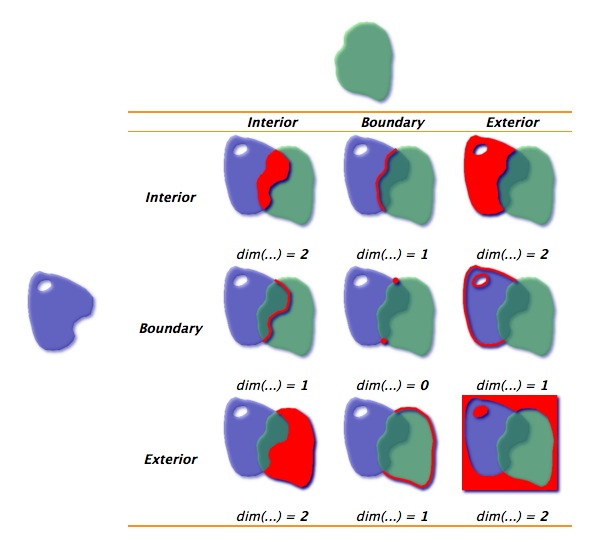
\includegraphics[width=0.5\textwidth]{figures/de9im3}
\end{frame}

\begin{frame}{Testing quality in original dataset...}{\footnote{\url{https://postgis.net/workshops/postgis-intro/de9im.html}}}
    \centering 
    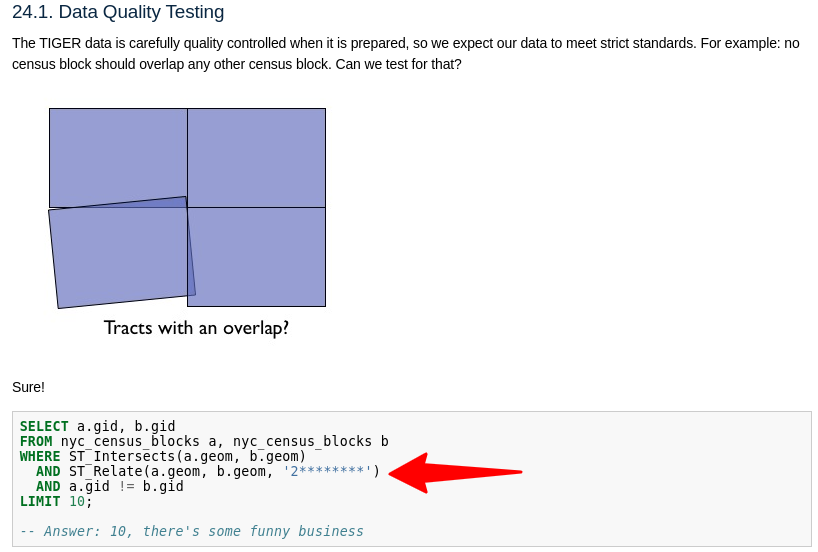
\includegraphics[width=0.75\textwidth]{figures/overlap}
\end{frame}

\begin{frame}{What is next...}
    \begin{itemize}
     \item Currently, I have problems during the execution in the cluster.  Some tasks do not finish and just keep working.  
     \item However, I have been able to finish on local mode with some sections of the data.
     \item I plan to test the full dataset by chunks of data until I can detect and fix the problem.
    \end{itemize}
\end{frame}

\end{document}
